\section{Numerical methods}\label{sec:numerics}
The figures show the radial law and the steps of its proof at finite
degrees, for nested sequences of random signs. This section records how
the roots and statistics behind them were computed, and how sensitive
they are to numerical error.
The limits that hold with probability one follow from the proofs in the
previous sections, and these proofs do not use the computations below.

We use 100 independent sequences of random signs at the degrees
$N=1000$, $3000$, $10000$, $30000$ and $100000$, and the block length is
$\lfloor N^{7/8}\rfloor$.
We use the 77 sequences whose roots were computed at all five base
degrees, all 421 intermediate degrees for 78 sequences at $N=1000$, and
the endpoint samples listed in Table~\ref{tab:numerical-coverage}.

\begin{table}[htbp]
\centering
\begin{tabular}{rrr}
\toprule
$N$ & Base samples & Endpoint samples\\
\midrule
$1000$ & 92 & 78\\
$3000$ & 92 & 58\\
$10000$ & 92 & 57\\
$30000$ & 91 & 53\\
$100000$ & 77 & 27\\
\bottomrule
\end{tabular}
\caption{Completed base samples and endpoint samples, at the degree
$N+\lfloor N^{7/8}\rfloor$. The $N=1000$ samples include every
intermediate degree.}
\label{tab:numerical-coverage}
\end{table}

The roots were computed with MPSolve~\cite{BiniRobol2014}, or, at the
degrees 1210 and 1421 of Figure~\ref{fig:root-matching}, with a
companion-matrix eigensolver, and then refined by Newton's method.
The residuals were checked by independent evaluation, and the normalized
residual $|f_N(z)|/\sum_{k=0}^N|z|^k$ is below $3\times10^{-14}$ at every
degree.

We determine the roots at $1$ and $-1$, with their multiplicities, by exact
integer division.
For the remaining roots, the band $\bigl||z|-1\bigr|\le10^{-9}$ yields a
sensitivity interval, whose two endpoints count every root in that band as
outside or inside the disk.
We check the counting procedure by direct evaluation and on polynomials
with known boundary roots.
Over all base samples, the numbers of the remaining roots in this band
are $0,0,2,28,284$, in increasing degree order, and they belong to
$0,0,1,12,61$ polynomials, respectively.
Thus the largest unnormalized sensitivity intervals have widths $0,0,2,4,14$.

We compute the angular occupations and the logarithmic integral on a
shifted FFT grid.
Doubling the grid changes the logarithmic average by at most
$4\times10^{-4}$ and the occupation by at most $2\times10^{-3}$.

The profile and root-count comparisons use the 77 sequences above, and
the angular comparisons use all 100.
The residuals and grid comparisons quantify numerical sensitivity rather
than interval certification.
The bands and intervals in the figures are pointwise 95\% percentile
intervals from 2000 bootstrap draws of whole sequences.
Figure~\ref{fig:radial-profile} compares the empirical profile
$\widehat\Phi_N(x)=\nu_N(1+x/N)/N$ with $\Phi(x)$.
Log--log fits for each statistic, which describe only the measured range,
are in \path{numerics/publication/STATISTICS.md} of the
repository~\cite{FormalCompanion2026}.

\begin{figure}[t]
\centering
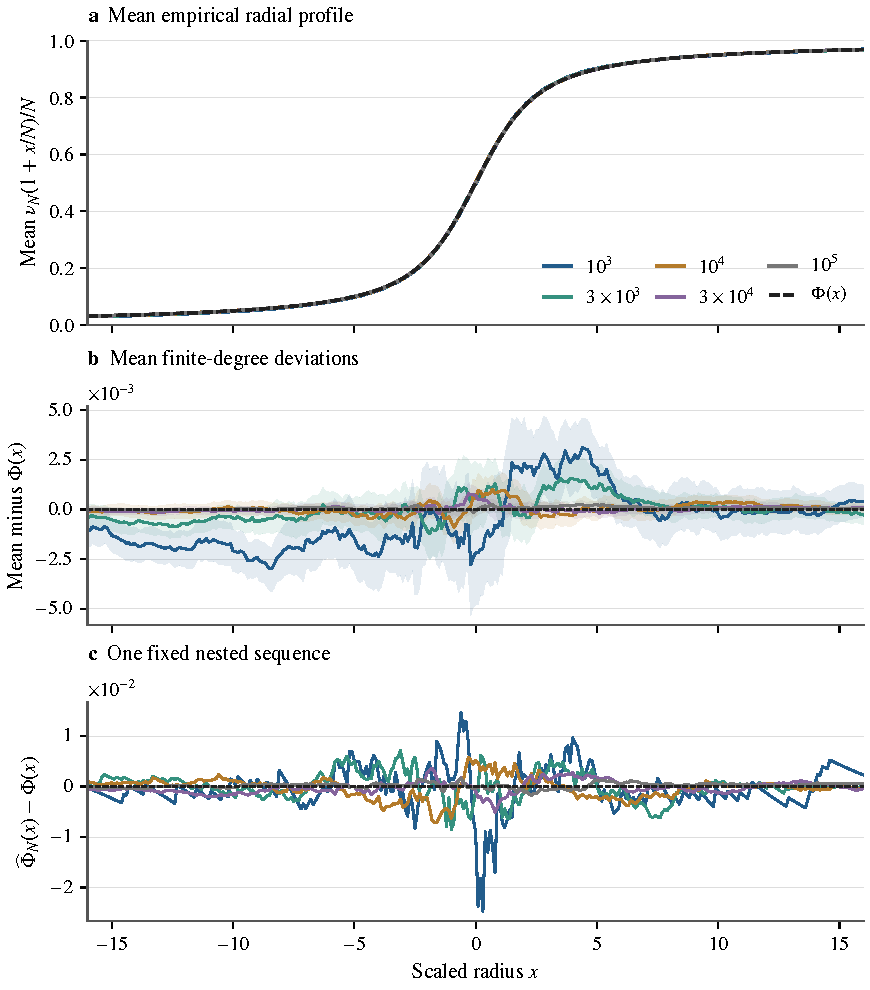
\includegraphics[height=0.6\textheight]{../numerics/publication/figures/radial-profile.pdf}
\caption{Mean empirical radial profile over 77 sequences at five degrees, which
cannot be distinguished from $\Phi$ (a), and its deviations (b, c).}
\label{fig:radial-profile}
\end{figure}

